% Options for packages loaded elsewhere
% Options for packages loaded elsewhere
\PassOptionsToPackage{unicode}{hyperref}
\PassOptionsToPackage{hyphens}{url}
\PassOptionsToPackage{dvipsnames,svgnames,x11names}{xcolor}
%
\documentclass[
  12pt,
]{article}
\usepackage{xcolor}
\usepackage[margin=1in]{geometry}
\usepackage{amsmath,amssymb}
\setcounter{secnumdepth}{-\maxdimen} % remove section numbering
\usepackage{iftex}
\ifPDFTeX
  \usepackage[T1]{fontenc}
  \usepackage[utf8]{inputenc}
  \usepackage{textcomp} % provide euro and other symbols
\else % if luatex or xetex
  \usepackage{unicode-math} % this also loads fontspec
  \defaultfontfeatures{Scale=MatchLowercase}
  \defaultfontfeatures[\rmfamily]{Ligatures=TeX,Scale=1}
\fi
\usepackage{lmodern}
\ifPDFTeX\else
  % xetex/luatex font selection
\fi
% Use upquote if available, for straight quotes in verbatim environments
\IfFileExists{upquote.sty}{\usepackage{upquote}}{}
\IfFileExists{microtype.sty}{% use microtype if available
  \usepackage[]{microtype}
  \UseMicrotypeSet[protrusion]{basicmath} % disable protrusion for tt fonts
}{}
\makeatletter
\@ifundefined{KOMAClassName}{% if non-KOMA class
  \IfFileExists{parskip.sty}{%
    \usepackage{parskip}
  }{% else
    \setlength{\parindent}{0pt}
    \setlength{\parskip}{6pt plus 2pt minus 1pt}}
}{% if KOMA class
  \KOMAoptions{parskip=half}}
\makeatother
% Make \paragraph and \subparagraph free-standing
\makeatletter
\ifx\paragraph\undefined\else
  \let\oldparagraph\paragraph
  \renewcommand{\paragraph}{
    \@ifstar
      \xxxParagraphStar
      \xxxParagraphNoStar
  }
  \newcommand{\xxxParagraphStar}[1]{\oldparagraph*{#1}\mbox{}}
  \newcommand{\xxxParagraphNoStar}[1]{\oldparagraph{#1}\mbox{}}
\fi
\ifx\subparagraph\undefined\else
  \let\oldsubparagraph\subparagraph
  \renewcommand{\subparagraph}{
    \@ifstar
      \xxxSubParagraphStar
      \xxxSubParagraphNoStar
  }
  \newcommand{\xxxSubParagraphStar}[1]{\oldsubparagraph*{#1}\mbox{}}
  \newcommand{\xxxSubParagraphNoStar}[1]{\oldsubparagraph{#1}\mbox{}}
\fi
\makeatother

\usepackage{color}
\usepackage{fancyvrb}
\newcommand{\VerbBar}{|}
\newcommand{\VERB}{\Verb[commandchars=\\\{\}]}
\DefineVerbatimEnvironment{Highlighting}{Verbatim}{commandchars=\\\{\}}
% Add ',fontsize=\small' for more characters per line
\usepackage{framed}
\definecolor{shadecolor}{RGB}{241,243,245}
\newenvironment{Shaded}{\begin{snugshade}}{\end{snugshade}}
\newcommand{\AlertTok}[1]{\textcolor[rgb]{0.68,0.00,0.00}{#1}}
\newcommand{\AnnotationTok}[1]{\textcolor[rgb]{0.37,0.37,0.37}{#1}}
\newcommand{\AttributeTok}[1]{\textcolor[rgb]{0.40,0.45,0.13}{#1}}
\newcommand{\BaseNTok}[1]{\textcolor[rgb]{0.68,0.00,0.00}{#1}}
\newcommand{\BuiltInTok}[1]{\textcolor[rgb]{0.00,0.23,0.31}{#1}}
\newcommand{\CharTok}[1]{\textcolor[rgb]{0.13,0.47,0.30}{#1}}
\newcommand{\CommentTok}[1]{\textcolor[rgb]{0.37,0.37,0.37}{#1}}
\newcommand{\CommentVarTok}[1]{\textcolor[rgb]{0.37,0.37,0.37}{\textit{#1}}}
\newcommand{\ConstantTok}[1]{\textcolor[rgb]{0.56,0.35,0.01}{#1}}
\newcommand{\ControlFlowTok}[1]{\textcolor[rgb]{0.00,0.23,0.31}{\textbf{#1}}}
\newcommand{\DataTypeTok}[1]{\textcolor[rgb]{0.68,0.00,0.00}{#1}}
\newcommand{\DecValTok}[1]{\textcolor[rgb]{0.68,0.00,0.00}{#1}}
\newcommand{\DocumentationTok}[1]{\textcolor[rgb]{0.37,0.37,0.37}{\textit{#1}}}
\newcommand{\ErrorTok}[1]{\textcolor[rgb]{0.68,0.00,0.00}{#1}}
\newcommand{\ExtensionTok}[1]{\textcolor[rgb]{0.00,0.23,0.31}{#1}}
\newcommand{\FloatTok}[1]{\textcolor[rgb]{0.68,0.00,0.00}{#1}}
\newcommand{\FunctionTok}[1]{\textcolor[rgb]{0.28,0.35,0.67}{#1}}
\newcommand{\ImportTok}[1]{\textcolor[rgb]{0.00,0.46,0.62}{#1}}
\newcommand{\InformationTok}[1]{\textcolor[rgb]{0.37,0.37,0.37}{#1}}
\newcommand{\KeywordTok}[1]{\textcolor[rgb]{0.00,0.23,0.31}{\textbf{#1}}}
\newcommand{\NormalTok}[1]{\textcolor[rgb]{0.00,0.23,0.31}{#1}}
\newcommand{\OperatorTok}[1]{\textcolor[rgb]{0.37,0.37,0.37}{#1}}
\newcommand{\OtherTok}[1]{\textcolor[rgb]{0.00,0.23,0.31}{#1}}
\newcommand{\PreprocessorTok}[1]{\textcolor[rgb]{0.68,0.00,0.00}{#1}}
\newcommand{\RegionMarkerTok}[1]{\textcolor[rgb]{0.00,0.23,0.31}{#1}}
\newcommand{\SpecialCharTok}[1]{\textcolor[rgb]{0.37,0.37,0.37}{#1}}
\newcommand{\SpecialStringTok}[1]{\textcolor[rgb]{0.13,0.47,0.30}{#1}}
\newcommand{\StringTok}[1]{\textcolor[rgb]{0.13,0.47,0.30}{#1}}
\newcommand{\VariableTok}[1]{\textcolor[rgb]{0.07,0.07,0.07}{#1}}
\newcommand{\VerbatimStringTok}[1]{\textcolor[rgb]{0.13,0.47,0.30}{#1}}
\newcommand{\WarningTok}[1]{\textcolor[rgb]{0.37,0.37,0.37}{\textit{#1}}}

\usepackage{longtable,booktabs,array}
\usepackage{calc} % for calculating minipage widths
% Correct order of tables after \paragraph or \subparagraph
\usepackage{etoolbox}
\makeatletter
\patchcmd\longtable{\par}{\if@noskipsec\mbox{}\fi\par}{}{}
\makeatother
% Allow footnotes in longtable head/foot
\IfFileExists{footnotehyper.sty}{\usepackage{footnotehyper}}{\usepackage{footnote}}
\makesavenoteenv{longtable}
\usepackage{graphicx}
\makeatletter
\newsavebox\pandoc@box
\newcommand*\pandocbounded[1]{% scales image to fit in text height/width
  \sbox\pandoc@box{#1}%
  \Gscale@div\@tempa{\textheight}{\dimexpr\ht\pandoc@box+\dp\pandoc@box\relax}%
  \Gscale@div\@tempb{\linewidth}{\wd\pandoc@box}%
  \ifdim\@tempb\p@<\@tempa\p@\let\@tempa\@tempb\fi% select the smaller of both
  \ifdim\@tempa\p@<\p@\scalebox{\@tempa}{\usebox\pandoc@box}%
  \else\usebox{\pandoc@box}%
  \fi%
}
% Set default figure placement to htbp
\def\fps@figure{htbp}
\makeatother


% definitions for citeproc citations
\NewDocumentCommand\citeproctext{}{}
\NewDocumentCommand\citeproc{mm}{%
  \begingroup\def\citeproctext{#2}\cite{#1}\endgroup}
\makeatletter
 % allow citations to break across lines
 \let\@cite@ofmt\@firstofone
 % avoid brackets around text for \cite:
 \def\@biblabel#1{}
 \def\@cite#1#2{{#1\if@tempswa , #2\fi}}
\makeatother
\newlength{\cslhangindent}
\setlength{\cslhangindent}{1.5em}
\newlength{\csllabelwidth}
\setlength{\csllabelwidth}{3em}
\newenvironment{CSLReferences}[2] % #1 hanging-indent, #2 entry-spacing
 {\begin{list}{}{%
  \setlength{\itemindent}{0pt}
  \setlength{\leftmargin}{0pt}
  \setlength{\parsep}{0pt}
  % turn on hanging indent if param 1 is 1
  \ifodd #1
   \setlength{\leftmargin}{\cslhangindent}
   \setlength{\itemindent}{-1\cslhangindent}
  \fi
  % set entry spacing
  \setlength{\itemsep}{#2\baselineskip}}}
 {\end{list}}
\usepackage{calc}
\newcommand{\CSLBlock}[1]{\hfill\break\parbox[t]{\linewidth}{\strut\ignorespaces#1\strut}}
\newcommand{\CSLLeftMargin}[1]{\parbox[t]{\csllabelwidth}{\strut#1\strut}}
\newcommand{\CSLRightInline}[1]{\parbox[t]{\linewidth - \csllabelwidth}{\strut#1\strut}}
\newcommand{\CSLIndent}[1]{\hspace{\cslhangindent}#1}



\setlength{\emergencystretch}{3em} % prevent overfull lines

\providecommand{\tightlist}{%
  \setlength{\itemsep}{0pt}\setlength{\parskip}{0pt}}



 


\usepackage{float}
\usepackage{tabularray}
\usepackage[normalem]{ulem}
\usepackage{graphicx}
\usepackage{rotating}
\UseTblrLibrary{booktabs}
\UseTblrLibrary{siunitx}
\NewTableCommand{\tinytableDefineColor}[3]{\definecolor{#1}{#2}{#3}}
\newcommand{\tinytableTabularrayUnderline}[1]{\underline{#1}}
\newcommand{\tinytableTabularrayStrikeout}[1]{\sout{#1}}
\makeatletter
\@ifpackageloaded{caption}{}{\usepackage{caption}}
\AtBeginDocument{%
\ifdefined\contentsname
  \renewcommand*\contentsname{Table of contents}
\else
  \newcommand\contentsname{Table of contents}
\fi
\ifdefined\listfigurename
  \renewcommand*\listfigurename{List of Figures}
\else
  \newcommand\listfigurename{List of Figures}
\fi
\ifdefined\listtablename
  \renewcommand*\listtablename{List of Tables}
\else
  \newcommand\listtablename{List of Tables}
\fi
\ifdefined\figurename
  \renewcommand*\figurename{Figure}
\else
  \newcommand\figurename{Figure}
\fi
\ifdefined\tablename
  \renewcommand*\tablename{Table}
\else
  \newcommand\tablename{Table}
\fi
}
\@ifpackageloaded{float}{}{\usepackage{float}}
\floatstyle{ruled}
\@ifundefined{c@chapter}{\newfloat{codelisting}{h}{lop}}{\newfloat{codelisting}{h}{lop}[chapter]}
\floatname{codelisting}{Listing}
\newcommand*\listoflistings{\listof{codelisting}{List of Listings}}
\makeatother
\makeatletter
\makeatother
\makeatletter
\@ifpackageloaded{caption}{}{\usepackage{caption}}
\@ifpackageloaded{subcaption}{}{\usepackage{subcaption}}
\makeatother
\usepackage{bookmark}
\IfFileExists{xurl.sty}{\usepackage{xurl}}{} % add URL line breaks if available
\urlstyle{same}
\hypersetup{
  pdftitle={Quarto template},
  pdfauthor={Jozef (ultimate nerd) Rivest},
  colorlinks=true,
  linkcolor={blue},
  filecolor={Maroon},
  citecolor={Blue},
  urlcolor={Blue},
  pdfcreator={LaTeX via pandoc}}


\title{Quarto template}
\author{Jozef (ultimate nerd) Rivest}
\date{October 16, 2025}
\begin{document}
\maketitle


This document provides a short introduction to Quarto. A few tips are
highlighted all along the file. If you have any questions, feel free to
ask me, or to refer to \href{https://quarto.org/docs/guide/}{Quarto
guide}. The best way to learn from it is either to try to replicate some
parts, or to change some parts and see how the output changed.

Have fun!

\newpage{}

\section{First level header}\label{first-level-header}

(Svolik 2012)

Svolik (2012)

\begin{Shaded}
\begin{Highlighting}[]
\NormalTok{dat }\OtherTok{\textless{}{-}}\NormalTok{ mtcars}

\FunctionTok{hist}\NormalTok{(dat}\SpecialCharTok{$}\NormalTok{cyl)}
\end{Highlighting}
\end{Shaded}

\pandocbounded{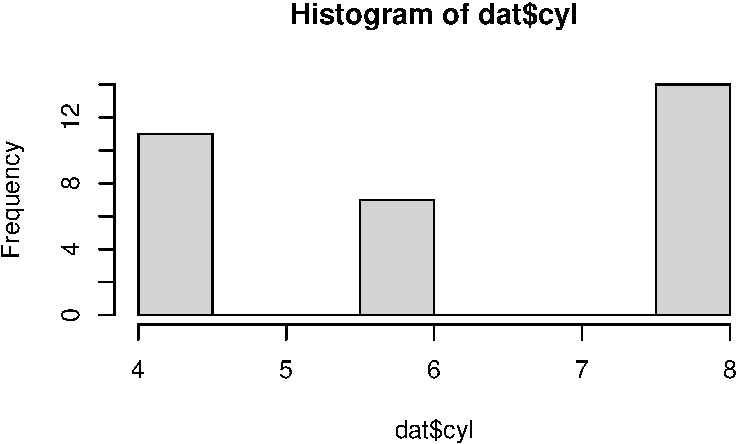
\includegraphics[keepaspectratio]{test_files/figure-pdf/unnamed-chunk-1-1.pdf}}

\begin{Shaded}
\begin{Highlighting}[]
\FunctionTok{library}\NormalTok{(tinytable) }\CommentTok{\# Super nice package for table!}

\FunctionTok{tt}\NormalTok{(dat)}
\end{Highlighting}
\end{Shaded}

\begin{table}
\centering
\begin{tblr}[         %% tabularray outer open
]                     %% tabularray outer close
{                     %% tabularray inner open
colspec={Q[]Q[]Q[]Q[]Q[]Q[]Q[]Q[]Q[]Q[]Q[]},
}                     %% tabularray inner close
\toprule
mpg & cyl & disp & hp & drat & wt & qsec & vs & am & gear & carb \\ \midrule %% TinyTableHeader
21.0 & 6 & 160.0 & 110 & 3.90 & 2.620 & 16.46 & 0 & 1 & 4 & 4 \\
21.0 & 6 & 160.0 & 110 & 3.90 & 2.875 & 17.02 & 0 & 1 & 4 & 4 \\
22.8 & 4 & 108.0 & 93 & 3.85 & 2.320 & 18.61 & 1 & 1 & 4 & 1 \\
21.4 & 6 & 258.0 & 110 & 3.08 & 3.215 & 19.44 & 1 & 0 & 3 & 1 \\
18.7 & 8 & 360.0 & 175 & 3.15 & 3.440 & 17.02 & 0 & 0 & 3 & 2 \\
18.1 & 6 & 225.0 & 105 & 2.76 & 3.460 & 20.22 & 1 & 0 & 3 & 1 \\
14.3 & 8 & 360.0 & 245 & 3.21 & 3.570 & 15.84 & 0 & 0 & 3 & 4 \\
24.4 & 4 & 146.7 & 62 & 3.69 & 3.190 & 20.00 & 1 & 0 & 4 & 2 \\
22.8 & 4 & 140.8 & 95 & 3.92 & 3.150 & 22.90 & 1 & 0 & 4 & 2 \\
19.2 & 6 & 167.6 & 123 & 3.92 & 3.440 & 18.30 & 1 & 0 & 4 & 4 \\
17.8 & 6 & 167.6 & 123 & 3.92 & 3.440 & 18.90 & 1 & 0 & 4 & 4 \\
16.4 & 8 & 275.8 & 180 & 3.07 & 4.070 & 17.40 & 0 & 0 & 3 & 3 \\
17.3 & 8 & 275.8 & 180 & 3.07 & 3.730 & 17.60 & 0 & 0 & 3 & 3 \\
15.2 & 8 & 275.8 & 180 & 3.07 & 3.780 & 18.00 & 0 & 0 & 3 & 3 \\
10.4 & 8 & 472.0 & 205 & 2.93 & 5.250 & 17.98 & 0 & 0 & 3 & 4 \\
10.4 & 8 & 460.0 & 215 & 3.00 & 5.424 & 17.82 & 0 & 0 & 3 & 4 \\
14.7 & 8 & 440.0 & 230 & 3.23 & 5.345 & 17.42 & 0 & 0 & 3 & 4 \\
32.4 & 4 & 78.7 & 66 & 4.08 & 2.200 & 19.47 & 1 & 1 & 4 & 1 \\
30.4 & 4 & 75.7 & 52 & 4.93 & 1.615 & 18.52 & 1 & 1 & 4 & 2 \\
33.9 & 4 & 71.1 & 65 & 4.22 & 1.835 & 19.90 & 1 & 1 & 4 & 1 \\
21.5 & 4 & 120.1 & 97 & 3.70 & 2.465 & 20.01 & 1 & 0 & 3 & 1 \\
15.5 & 8 & 318.0 & 150 & 2.76 & 3.520 & 16.87 & 0 & 0 & 3 & 2 \\
15.2 & 8 & 304.0 & 150 & 3.15 & 3.435 & 17.30 & 0 & 0 & 3 & 2 \\
13.3 & 8 & 350.0 & 245 & 3.73 & 3.840 & 15.41 & 0 & 0 & 3 & 4 \\
19.2 & 8 & 400.0 & 175 & 3.08 & 3.845 & 17.05 & 0 & 0 & 3 & 2 \\
27.3 & 4 & 79.0 & 66 & 4.08 & 1.935 & 18.90 & 1 & 1 & 4 & 1 \\
26.0 & 4 & 120.3 & 91 & 4.43 & 2.140 & 16.70 & 0 & 1 & 5 & 2 \\
30.4 & 4 & 95.1 & 113 & 3.77 & 1.513 & 16.90 & 1 & 1 & 5 & 2 \\
15.8 & 8 & 351.0 & 264 & 4.22 & 3.170 & 14.50 & 0 & 1 & 5 & 4 \\
19.7 & 6 & 145.0 & 175 & 3.62 & 2.770 & 15.50 & 0 & 1 & 5 & 6 \\
15.0 & 8 & 301.0 & 335 & 3.54 & 3.570 & 14.60 & 0 & 1 & 5 & 8 \\
21.4 & 4 & 121.0 & 109 & 4.11 & 2.780 & 18.60 & 1 & 1 & 4 & 2 \\
\bottomrule
\end{tblr}
\end{table}

You can insert math equations the same way you would do in \LaTeX.
Either with the double dollar sign, or using
\texttt{begin\{equation\}\ end\{equation\}} in a \LaTeX chunk.

\[
P(A|B) = \frac{P(B|A)P(A)}{P(B|A)P(A) + P(B|A^c)P(A^c)}
\]

\begin{equation}
P(A|B) = \frac{P(B|A)P(A)}{P(B|A)P(A) + P(B|A^c)P(A^c)}
\end{equation}

\newpage{}

\section{References}\label{references}

\phantomsection\label{refs}
\begin{CSLReferences}{1}{0}
\bibitem[\citeproctext]{ref-svolik2012}
Svolik, Milan W. 2012. \emph{The Politics of Authoritarian Rule}. 1st
ed. Cambridge University Press.
\url{https://doi.org/10.1017/CBO9781139176040}.

\end{CSLReferences}

\newpage{}

\section{Appendix}\label{appendix}

Sometimes, packages print errors, messages, and warnings. To silence
them, you can add the following in the code chunk (see the second code
chunk below)

\begin{Shaded}
\begin{Highlighting}[]
\FunctionTok{library}\NormalTok{(tidyverse)}
\end{Highlighting}
\end{Shaded}

\begin{verbatim}
-- Attaching core tidyverse packages ------------------------ tidyverse 2.0.0 --
v dplyr     1.1.4     v readr     2.1.5
v forcats   1.0.1     v stringr   1.5.2
v ggplot2   4.0.0     v tibble    3.3.0
v lubridate 1.9.4     v tidyr     1.3.1
v purrr     1.1.0     
-- Conflicts ------------------------------------------ tidyverse_conflicts() --
x dplyr::filter()       masks stats::filter()
x dplyr::lag()          masks stats::lag()
x ggplot2::theme_void() masks tinytable::theme_void()
i Use the conflicted package (<http://conflicted.r-lib.org/>) to force all conflicts to become errors
\end{verbatim}

\begin{Shaded}
\begin{Highlighting}[]
\FunctionTok{library}\NormalTok{(tidyverse)}
\end{Highlighting}
\end{Shaded}

\newpage{}

\section{Appendix 2}\label{appendix-2}

If you want to hide the code, you can add \texttt{echo:\ false} to the
code chunk:

\begin{table}
\centering
\begin{tblr}[         %% tabularray outer open
]                     %% tabularray outer close
{                     %% tabularray inner open
colspec={Q[]Q[]Q[]Q[]Q[]Q[]Q[]Q[]Q[]Q[]Q[]},
}                     %% tabularray inner close
\toprule
mpg & cyl & disp & hp & drat & wt & qsec & vs & am & gear & carb \\ \midrule %% TinyTableHeader
21.0 & 6 & 160.0 & 110 & 3.90 & 2.620 & 16.46 & 0 & 1 & 4 & 4 \\
21.0 & 6 & 160.0 & 110 & 3.90 & 2.875 & 17.02 & 0 & 1 & 4 & 4 \\
22.8 & 4 & 108.0 & 93 & 3.85 & 2.320 & 18.61 & 1 & 1 & 4 & 1 \\
21.4 & 6 & 258.0 & 110 & 3.08 & 3.215 & 19.44 & 1 & 0 & 3 & 1 \\
18.7 & 8 & 360.0 & 175 & 3.15 & 3.440 & 17.02 & 0 & 0 & 3 & 2 \\
18.1 & 6 & 225.0 & 105 & 2.76 & 3.460 & 20.22 & 1 & 0 & 3 & 1 \\
14.3 & 8 & 360.0 & 245 & 3.21 & 3.570 & 15.84 & 0 & 0 & 3 & 4 \\
24.4 & 4 & 146.7 & 62 & 3.69 & 3.190 & 20.00 & 1 & 0 & 4 & 2 \\
22.8 & 4 & 140.8 & 95 & 3.92 & 3.150 & 22.90 & 1 & 0 & 4 & 2 \\
19.2 & 6 & 167.6 & 123 & 3.92 & 3.440 & 18.30 & 1 & 0 & 4 & 4 \\
17.8 & 6 & 167.6 & 123 & 3.92 & 3.440 & 18.90 & 1 & 0 & 4 & 4 \\
16.4 & 8 & 275.8 & 180 & 3.07 & 4.070 & 17.40 & 0 & 0 & 3 & 3 \\
17.3 & 8 & 275.8 & 180 & 3.07 & 3.730 & 17.60 & 0 & 0 & 3 & 3 \\
15.2 & 8 & 275.8 & 180 & 3.07 & 3.780 & 18.00 & 0 & 0 & 3 & 3 \\
10.4 & 8 & 472.0 & 205 & 2.93 & 5.250 & 17.98 & 0 & 0 & 3 & 4 \\
10.4 & 8 & 460.0 & 215 & 3.00 & 5.424 & 17.82 & 0 & 0 & 3 & 4 \\
14.7 & 8 & 440.0 & 230 & 3.23 & 5.345 & 17.42 & 0 & 0 & 3 & 4 \\
32.4 & 4 & 78.7 & 66 & 4.08 & 2.200 & 19.47 & 1 & 1 & 4 & 1 \\
30.4 & 4 & 75.7 & 52 & 4.93 & 1.615 & 18.52 & 1 & 1 & 4 & 2 \\
33.9 & 4 & 71.1 & 65 & 4.22 & 1.835 & 19.90 & 1 & 1 & 4 & 1 \\
21.5 & 4 & 120.1 & 97 & 3.70 & 2.465 & 20.01 & 1 & 0 & 3 & 1 \\
15.5 & 8 & 318.0 & 150 & 2.76 & 3.520 & 16.87 & 0 & 0 & 3 & 2 \\
15.2 & 8 & 304.0 & 150 & 3.15 & 3.435 & 17.30 & 0 & 0 & 3 & 2 \\
13.3 & 8 & 350.0 & 245 & 3.73 & 3.840 & 15.41 & 0 & 0 & 3 & 4 \\
19.2 & 8 & 400.0 & 175 & 3.08 & 3.845 & 17.05 & 0 & 0 & 3 & 2 \\
27.3 & 4 & 79.0 & 66 & 4.08 & 1.935 & 18.90 & 1 & 1 & 4 & 1 \\
26.0 & 4 & 120.3 & 91 & 4.43 & 2.140 & 16.70 & 0 & 1 & 5 & 2 \\
30.4 & 4 & 95.1 & 113 & 3.77 & 1.513 & 16.90 & 1 & 1 & 5 & 2 \\
15.8 & 8 & 351.0 & 264 & 4.22 & 3.170 & 14.50 & 0 & 1 & 5 & 4 \\
19.7 & 6 & 145.0 & 175 & 3.62 & 2.770 & 15.50 & 0 & 1 & 5 & 6 \\
15.0 & 8 & 301.0 & 335 & 3.54 & 3.570 & 14.60 & 0 & 1 & 5 & 8 \\
21.4 & 4 & 121.0 & 109 & 4.11 & 2.780 & 18.60 & 1 & 1 & 4 & 2 \\
\bottomrule
\end{tblr}
\end{table}




\end{document}
